% Chapter 3

\chapter{General Polynomial Chaos}
Die hier aufgezeigte Einführung in das general Polynomial Chaos (gPC) ist angelehnt an Xiu in \autocite{dongbinxiu2010}.
\section{Approximation von Zufallsvariablen}
Anhand des Beispiels \ref{bsp:hermitechaos} des Hermite-Chaos haben wir bereits gesehen, dass für gewisse Orthonormalbasen von Polynomen $\lbrace H_i\rbrace$ und Zufallsvariablen $Y$ mit passenden stochastischen Verteilungen die Beziehung
\[\langle H_i,H_j\rangle_{L_w^2(S)} =\E_Y \left[H_i(Y)H_j(Y)\right]=\delta_{ij}\]
erfüllt wird.
\begin{mathdef}[General Polynomial Chaos Basis]
\label{def:gpc}
Sei $Y$ eine reelle Zufallsvariable mit Verteilungsfunktion $F_Y(y)=P(Y\le y)$ und endlichen Momenten
\[\E\left[|Y|^{2m}\right]=\int |y|^{2m}dF_Y(y)<\infty,\quad m\in \N_0\]
Existieren Polynome $\Phi_i\in\Poly_i$ welche die Bedingung
\begin{equation}
\label{eqn:gpc_basicortho}
\E\left[\Phi_i(Y)\Phi_j(Y)\right]=\delta_{ij},\quad i,j\in\N_0
\end{equation}
erfüllen, so nennt man diese \emph{general Polynomial Chaos Basis Funktionen}.\\
Ist $Y$ stetig, so existiert eine Dichtefunktion $\rho>0$, so dass $dF_Y(y)=\rho(y)dy$ auf $I$. In diesem Fall lässt sich die Bedingung (\ref{eqn:gpc_basicortho}) schreiben als
\begin{equation}
\label{eqn:gpc_ortho}
\E\left[\Phi_i(Y)\Phi_j(Y)\right]=\int_I \Phi_i(y)\Phi_j(y)\rho(y)dy=\delta_{ij},\quad i,j\in\N_0
\end{equation}
\end{mathdef}
\begin{mathbem}
Betrachten wir die Orthogonalitätsbedingung (\ref{eqn:gpc_ortho}), so wird klar, dass diese direkt der Orthogonalität des Raumes $L_\rho^2(I)$ entspricht. Die Polynome erfüllen somit nach Satz \ref{threetermexist} eine Drei-Term-Rekursion und bilden eine Orthonormalbasis bezüglich $L_\rho^2(I)$.\\
Man beachte, dass die hier vorgenommene Normierung der Basis keine Beschränkung der Allgemeinheit darstellt. Gilt als Bedingung nur
\[\langle H_i,H_j\rangle_{L_w^2(S)} =\E_Y \left[H_i(Y)H_j(Y)\right]=\gamma_i\delta_{ij},\quad i,j\in\N_0,\gamma_i>0\]
so müssen die Polynome $H_i$ lediglich durch die Normalisierungskonstanten $\sqrt{\gamma_i}=\sqrt{\E\left[\Phi_i^2(Y)\right]}$ geteilt werden.\\
Ist $Y$ keine stetige sondern eine diskrete Zufallsvariable, so ändert sich die Notation und aus obigen Integralen würden Reihen, die Kernaussagen blieben aber dieselben. Wir werden jedoch im Folgenden stets stetige Zufallsvariablen verwenden.
\end{mathbem}
Eine Übersicht von einigen bekannten Verteilungen und Polynombasen ist in Tabelle \ref{table:chaos} gegeben. Details zu stetigen Verteilungen finden sich im Anhang \ref{AppendixA}.\\
\begin{center}
\begin{tabular}{c|ccc}
 & Verteilung von $Y$ & gPC Basispolynome & Träger \\ 
\hline 
Stetig & Normal & Hermite & $(-\infty,\infty)$ \\ 
 & Gamma & Laguerre & $[0,\infty)$ \\ 
 & Beta & Jacobi & $[-1,1]$ \\
 & Gleich & Legendre & $[-1,1]$ \\  
\hline 
Diskret & Poisson & Charlier & $\lbrace 0,1,2,\dots\rbrace$ \\ 
 & Binomial & Krawtchouk & $\lbrace 0,1,\dots,P\rbrace$ \\ 
 & Negativ Binomial & Meixner & $\lbrace 0,1,2,\dots\rbrace$ \\  
 & Hypergeometrisch & Hahn & $\lbrace 0,1,\dots,P\rbrace$
\label{table:chaos}
\end{tabular} 
\todo[inline]{Das hier als caption!}
gPC Beziehung zwischen orthogonalen Polynombasen und stochastischen Verteilungen. $P\in\N_0$ ist dabei ein beliebiger Parameter für gewisse diskrete Verteilungen.
\end{center}

Das Ziel ist es nun, mithilfe einer gPC Orthonormalbasis eine Funktion $f(Y)$ einer Zufallsvariablen $Y$ zu approximieren. Wir wollen nun einen Einblick dazu bekommen, was an dieser Stelle mit "`approximieren"' gemeint ist.
\begin{mathdef}[Starke gPC Konvergenz]
Sei $f(Y)$ eine Funktion einer Zufallsvariablen $Y$ mit Dichte $\rho_Y$ und Träger $I_Y$. Eine general Polynomial Chaos Approximation $f_M(Y)\in\Poly_N(Y)$ konvergiert in einem starken Sinne gegen $F(Y)$, wenn \[\norm{f(Y)-f_M(Y)}_{L_{\rho_Y}^2(I_Y)}\to 0\text{ für }{M\to\infty}\]
\end{mathdef}
Die starke gPC Konvergenz entspricht also direkt der in Kapitel \ref{sec:poly_approx} vorgestellten spektralen Konvergenz, entsprechend ist die Konvergenzordnung abhängig von der Glattheit der Funktion $f$. Ohne Beweis folgt aus der starken gPC Konvergenz auch die Konvergenz in Wahrscheinlichkeit und schlussendlich die Konvergenz in Verteilung.
\begin{mathbem}
Ist die Funktion $f$ oder ihre Abhängigkeit von der Zufallsvariablen $Y$ nicht konkret bekannt, sondern liegt diese beispielsweise nur als Verteilungsfunktion vor, so ist es dennoch möglich eine gPC Approximation in einem schwachen Sinne zu erhalten. Für Details sei auf \autocite[Kapitel 5.1.2]{dongbinxiu2010} verwiesen.\\
Ein illustratives Beispiel ist in Abbildung \ref{fig:gpcweakconv} gegeben. Dort verwenden wir die Bestapproximation bezüglich $L_\rho^2(-\infty,\infty)$, wobei $\rho$ die Dichtefunktion der Normalverteilung ist, die Orthonormalbasis aus den Hermite-Polynomen $H_k$ besteht und $Y$ eine normalverteilte Zufallsvariable ist. Es ist
\[f_M(Y)=P_M(f)=\sum_{m=0}^M\hat{f}_mH_m(Y), \quad \hat{f}_m=\E[f(Y)H_m(Y)]\]
die Bestapproximation an die Funktion $f(Y)$ in $\Poly_M(Y)$. Wir nehmen an, dass wir nur die Verteilung von $Z=f(Y)$ kennen und $Z\sim\text{Beta}(0.2,3.)$ in $[-1,1]$.\\
Dann tritt bei der Berechnung von $\E[ZH_m(Y)]$ eine Schwierigkeit auf: es ist in dieser Form nicht möglich den Erwartungswert zu berechnen, da die Zufallsvariablen $Z$ und $H_m(Y)$ zu verschiedenen Wahrscheinlichkeitsräumen gehören. Hierzu ist es nun hilfreich, mithilfe der Inversionsmethode die beiden Verteilungen auf einen gemeinsamen Wahrscheinlichkeitsraum $\mathcal{U}(0,1)$ zu "`normieren"'. Dann gilt
\[\hat{f}_m=\E_U\left[F_Z^{-1}(U)H_m(F_Y^{-1}(U))\right]=\int_0^1F_Z^{-1}(u)H_m(F_Y^{-1}(u))du\]
und $f_M(Y)$ konvergiert in Verteilung gegen $f(Y)$ für $M\to\infty$.
\begin{figure}[!htb]
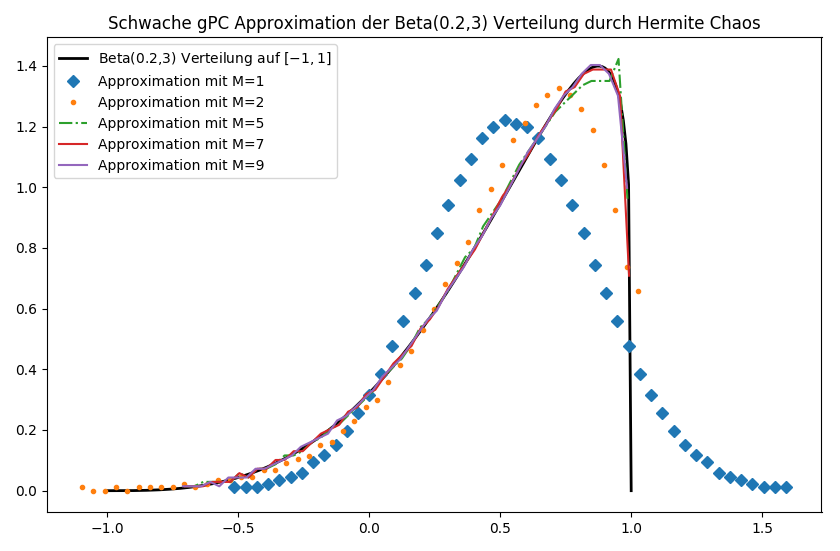
\includegraphics[width=\textwidth]{Figures/gpc_weak_convergence.png}
\caption{Schwache Konvergenz von Hermite gPC Approximation zu einer $\text{Beta}(0.2,3.)$ verteilten Zufallsvariablen. Dargestellt sind Approximationen an die Dichtefunktionen, welche über Histogramme von 50 gleich großen Intervallen angenähert werden.}
\label{fig:gpcweakconv}
\end{figure}
\end{mathbem}

\section{Mehrdimensionale Zufallsräume}
Wie bereits diskutiert, sei der Zufallsraum durch einen Zufallsvektor $Y=(Y_1,\dots,Y_N)^T$ mit stochastisch unabhängigen Komponenten $Y_i$ mit bekannter Verteilung vollständig parametrisiert. Als mehrdimensionale Erweiterung von Definition \ref{def:gpc} führen wir an dieser Stelle das multivariate gPC ein.
\begin{mathdef}[Multivariate gPC]
Sei $M\in\N_0$ der fest gewählte maximale Polynomgrad. Sei weiter $Y=(Y_1,\dots,Y_N)^T$ ein Zufallsvektor, dessen unabhängige Komponenten $Y_k$ eine gPC Basis $\lbrace \Phi_i^{(k)}\in\Poly_M(Y_k)|\quad i=1,\dots,M\rbrace$ besitzen. Ist $m=(m_1,\dots,m_N)\in\N_0^N$ ein Multi-Index mit $|m|=m_1+\dots+m_N$, so sind die $N$-variate gPC Basis Funktionen vom Grad $M$ definiert als 
\[\Phi_m(Y)=\Phi_{m_1}(Y_1)\cdot\ldots\cdot\Phi_{m_N}(Y_N),\quad 0\le |m|\le M\]
\end{mathdef}

\begin{mathbem}
Der von den multivariate gPC Funktionen aufgespannte Raum $\Poly_M^N$ ist der Raum aller Polynome vom Grad höchstens $M$ in $N$ Variablen
\[\Poly_M^N(Y)=\left\lbrace p\colon I_Y\to \R |\quad p(Y)=\sum_{|m|\le M}c_m\Phi_m(Y)\right\rbrace\]
Die Dimension des Raumes ist $\dim\Poly_M^N=\left(\frac{M+N}{M}\right)$.
\todo{Nicht frac sondern binomial...}
\end{mathbem}
\begin{proof}
Wir zeigen die zweite Aussage über die Dimension des Raumes. Dies ist ein konstruktiver Beweis, der dann gleichzeitig einen möglichen Algorithmus zur Generierung der Multi-Indices beschreibt.\\
Da die Monome $x^m=x_1^{m_1}\dots x_N^{m_N}$ für verschiedene $m=(m_1,\dots,m_N)$ linear unabhängig und erzeugend sind, ist die Aussage äquivalent zur Aussage
\[\frac{M+N}{M}=\#\lbrace m\in\N_0^N |\quad |m|\le M\rbrace\] 
Wir berechnen dazu $a_j=\#\lbrace m\in\N_0^N |\quad |m|=j\rbrace$ für $j=0,\dots,M$. Dazu überlegen wir uns, dass $a_j=\#\lbrace \overline{m}\in\N^N |\quad |\overline{m}|=j+N\rbrace$ wegen der Bijektion $m=(m_1,\dots,m_N)=(\overline{m}_1+1,\dots,\overline{m}_N+1)$. Wir wollen nun herausfinden, wieviele Zerlegungen der Zahl $j+N$ möglich sind und schreiben dazu symbolisch
\[\overline{m}=\underbrace{(1\_1\_1\_\dots 1\_1)}_{j+N\text{ Einsen getrennt von } j+N-1 \text{ Blanks}}\]
Um eine mögliche Darstellung zu bekommen, ersetzen wir $N-1$ Blanks durch ein Komma und die restlichen durch ein Plus, beispielsweise für $j=4,N=3$
\[(1+1+1,1,1+1+1+1+1)=(3,1,5)=\overline{m}\]
Dies sind exakt alle Möglichkeiten $N$ positive Zahlen deren Summe $j+N$ ist zu erhalten und es ist $a_j=\frac{j+N-1}{N-1}$.
Anschließend berechnen wir noch $\sum_{j=0}^M\frac{j+N-1}{N-1}=...$
\end{proof}
\todo[inline]{Suche schönere Variante für Trennsymbol von Mengen und ersetze für alle Vorkomnnise}
\todo[inline]{Spreche Sortierung der m an, das wir zukünftig m nicht als Multiindex sondern als Numerrierung auffassen und wie stark die Anzahl wächst (aber immer noch besser als full tensor)}